\documentclass{standalone}
\usepackage{tikz}
\usetikzlibrary{3d,arrows, calc, backgrounds, petri, positioning, shadows, shapes}


\tikzset{
	persp/.style={scale=3.0,x={(-0.8cm,-0.4cm)},y={(0.8cm,-0.4cm)}, z={(0cm,1cm)}},
	points/.style={fill=white,draw=black,thick}
	grid/.style={very thin,gray},
	axis/.style={->,ultra thick},
	cube/.style={thick, fill=black!15,opacity=0.5},
	cube hidden/.style={dashed},
	block/.style={
		rectangle, rounded corners,
		draw=black!80,
		fill=black!10, fill opacity=0.5,
		text=black!90, text opacity=1.0,
    text height=1.5ex,
    text depth=.25ex,
    text width=6em,
    text centered
	}
}

\tikzstyle{class}			=[rectangle, rounded corners, draw=black, fill=blue!40, drop shadow, text centered, anchor=north, text=white,    text width=3cm]
\tikzstyle{module}		=[rectangle, rounded corners, draw=black, fill=red!40, 	drop shadow, text centered, anchor=north, text=white,    text width=3cm]
\tikzstyle{component}	=[rectangle, rounded corners, draw=black, fill=green,   drop shadow, text centered, anchor=north, text=black!90, text width=3cm]
\tikzstyle{single}		=[text height=1.5ex, text depth=0.25ex]
\tikzstyle{double}		=[text height=4.0ex, text depth=2.75ex]
\tikzstyle{triple}		=[text height=6.5ex, text depth=5.25ex]
\tikzstyle{quadru}		=[text height=9.0ex, text depth=7.75ex]
\newcommand*{\rootPath}{../}

\begin{document}
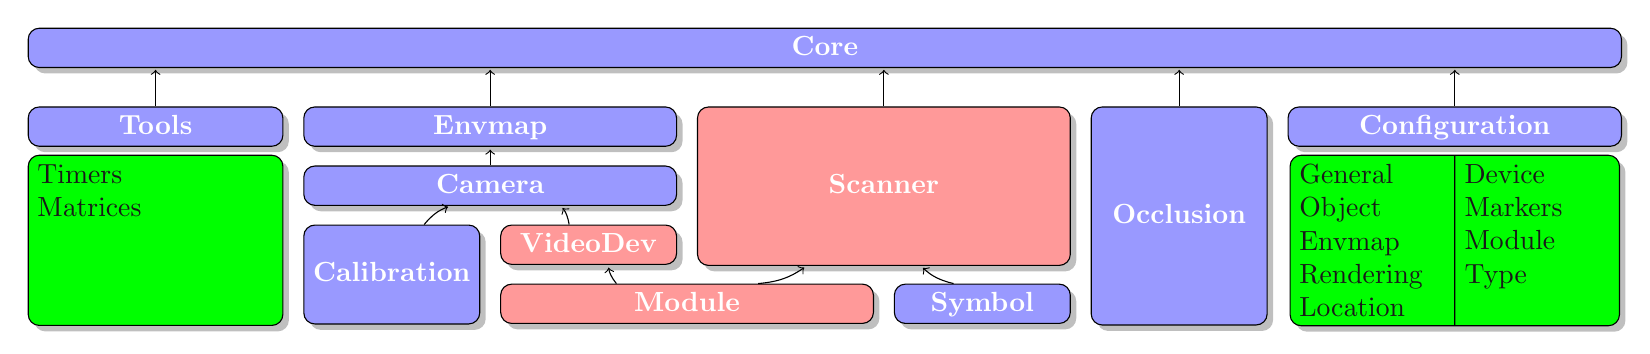
\begin{tikzpicture}[node distance=2cm]


	\node (Core)				[class, 		single, text width=20cm]			at (+0.00, +0.00)					{	\textbf{Core}						};
	\node (Tools)				[class,			single, text width=3cm]				at (-8.50, -1.00)					{	\textbf{Tools}					}			edge[post] (-8.50, -0.50) ;
	\node (ToolsDesc) 	[component,	below=0.1cm of Tools, text justified]
	{
		Timers\newline
		Matrices\newline
		\newline
		\newline
	};

	\node (Envmap)			[class,			single, text width=4.5cm]			at (-4.25, -1.00)					{	\textbf{Envmap}					}			edge[post] (-4.25, -0.50) ;
	\node (Camera)			[class,			single, text width=4.5cm]			at (-4.25, -1.75)					{	\textbf{Camera}					}			edge[post] (Envmap) ;
	\node (Scanner)			[module,		triple, text width=4.5cm]			at (+0.75, -1.00)					{	\textbf{Scanner}				}			edge[post] (+0.75, -0.50) ;

	\node (Calibration)	[class,			double, text width=2.0cm]			at (-5.50, -2.50)					{	\textbf{Calibration}		}			edge[post, bend left=15]	(Camera) ;
	\node (Video)				[module,		single, text width=2.0cm]			at (-3.00, -2.50)					{	\textbf{VideoDev}				}			edge[post, bend right=15]	(Camera) ;
	\node (Module)			[module,		single, text width=4.5cm]			at (-1.75, -3.25)					{	\textbf{Module}					}			edge[post, bend left=15]	(Video)
																																																													edge[post, bend right=15]	(Scanner) ;
	\node (Symbol)			[class,			single, text width=2.0cm]			at (+2.00, -3.25)					{	\textbf{Symbol}					}			edge[post, bend left=15]	(Scanner) ;

	\node (Occlusion)		[class,			quadru, text width=2cm]				at (+4.50, -1.00)					{	\textbf{Occlusion}			}			edge[post] (+4.50, -0.50) ;

	\node (Config)			[class,			single, text width=4cm]				at (+8.00, -1.00)					{	\textbf{Configuration}	}			edge[post] (+8.00, -0.50) ;
	\node (ConfigDesc) 	[component,	below=0.1cm of Config, text justified, rectangle split, rectangle split parts=2, rectangle split horizontal, text width=1.85cm]
	{
		General\newline
		Object\newline
		Envmap\newline
		Rendering\newline
		Location
		\nodepart{second}
		Device\newline
		Markers\newline
		Module\newline
		Type\newline
	};

\end{tikzpicture}
\end{document}